
%%%%%%%%%%%%%%%%%%%
%%% SVHN RESULTS
%%%%%%%%%%%%%%%%%%%
\begin{figure}[t]
\begin{center}\small
\setlength{\tabcolsep}{3pt}
		\subfigure[Mean IOU of various propagation methods.]
		{
			\begin{minipage}{0.58\textwidth}
				\label{fig:input-model}
				% \centering
				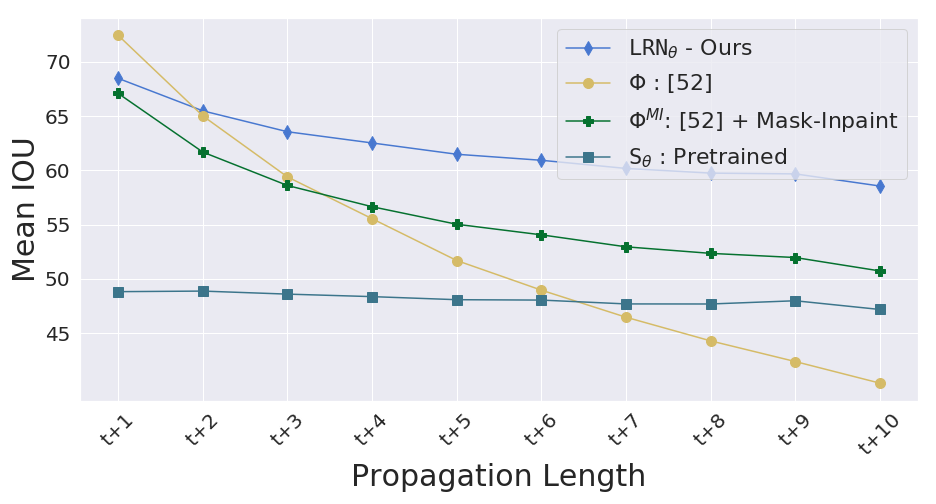
\includegraphics[width=1.0\linewidth]{figures/miou_apollo.png}
				\hfill
				\vfill
			\end{minipage}
		}
% \hspace{-1em}
% \vtop{
% \vspace{-1em}
\hfill
% \hbox{
% 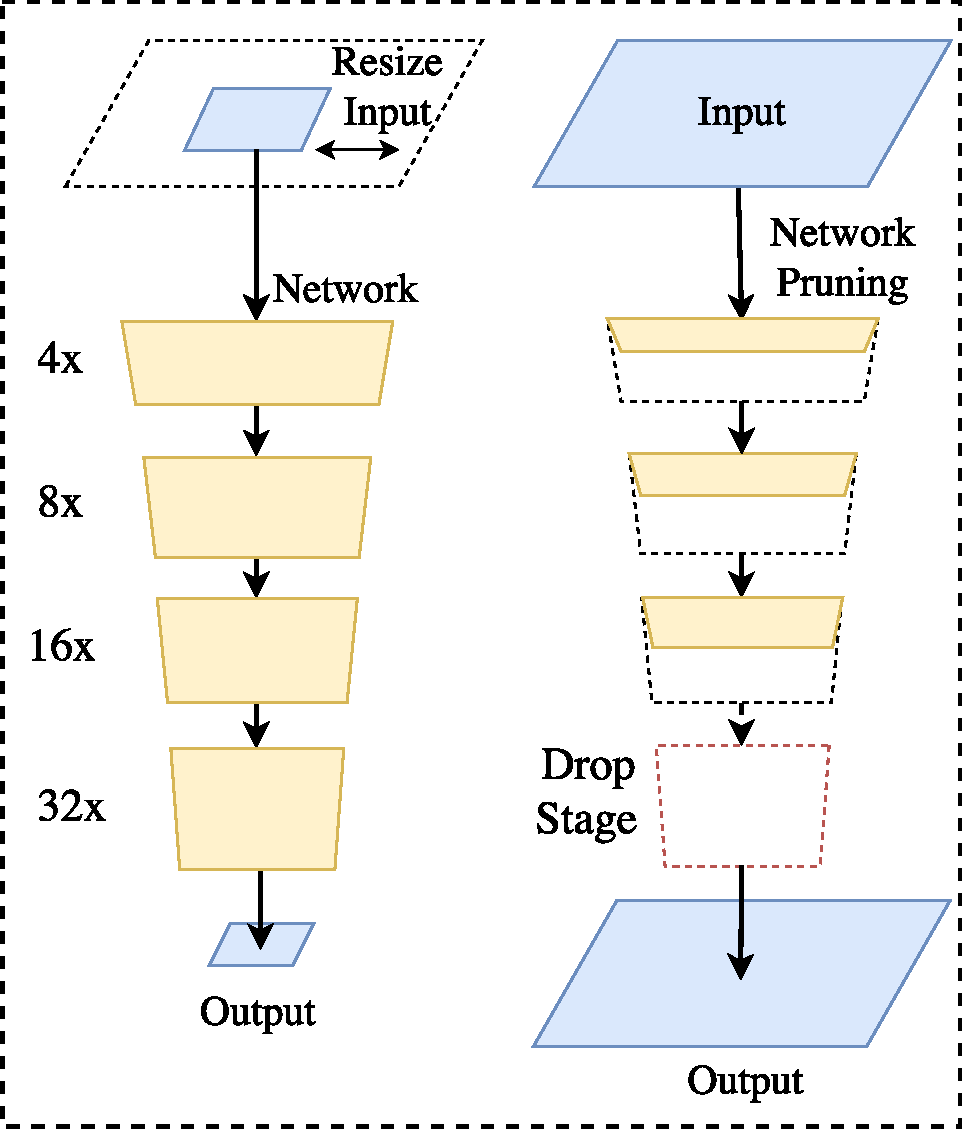
\includegraphics[width=0.6\textwidth]{figures/input_model.pdf}
		\subfigure[Qualitative Example]{
            \begin{minipage}{0.35\textwidth}
                \centering
				\label{fig:input-model}
				% \centering
				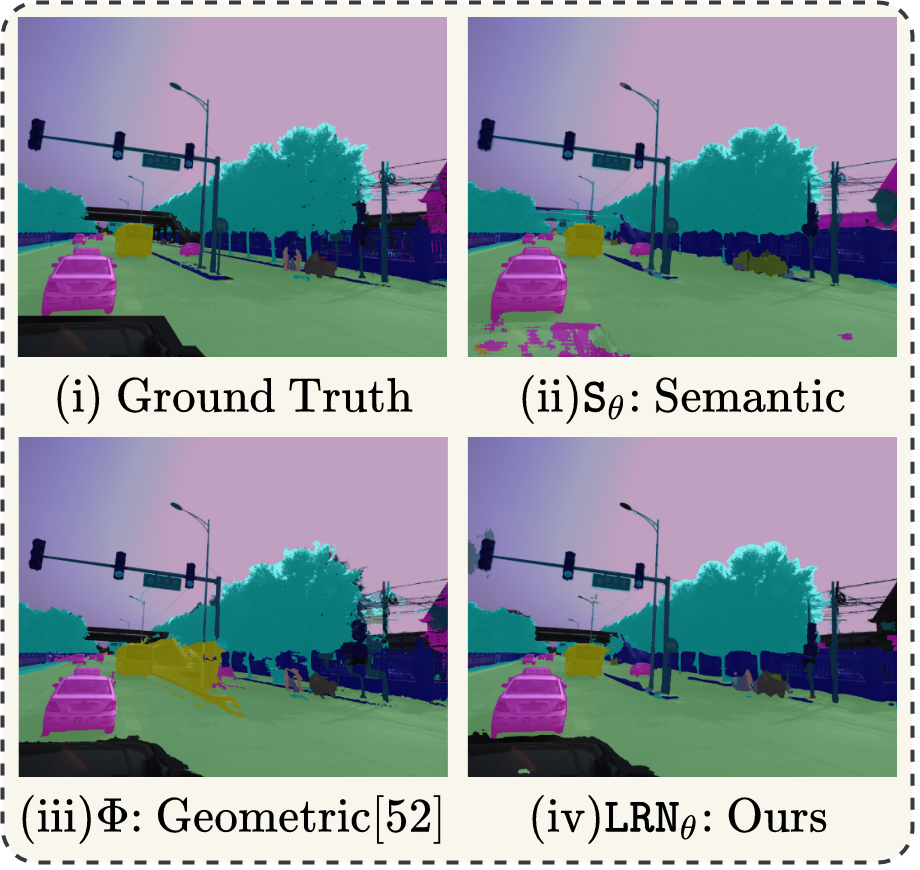
\includegraphics[width=1.0\linewidth]{figures/apollo_vis.png}
\end{minipage}
% }}%
}
\end{center}
\vspace{-1em}
\caption{\small \emph{(a)} We \textit{quantitatively} show that our method is significantly better than previous \textit{state-of-the-art} method. \emph{(b)} \cite{nvidia_cvpr19}, which uses geometric information is suspectible to poor warping, on the other hand generating pseudo-labels from semantic predictions (via network $\mathtt{S}_\theta$ poorly labels rare classes. Our method combines geometric and semantic information together, generating cleaner labels.}
\label{table:svhn}

		\vspace{-1em}
\end{figure}
